\chapter{Requirements analyse}\label{ch:requirements-analyse}

In dit hoofdstuk wordt er gekeken naar het op te lossen probleem en wie er gebaad bij is. Daarnaast wordt er gekeken welke eisen er gesteld zijn er welke priotisering er is gemaakt om aan deze eisen te voldoen.


\section{Huidige situatie}\label{sec:huid-sit}
De huidige situatie is dat er op dit moment geen concreet en centraal inzicht is in het gebruikt van externe bibliotheken en de kwetsbaarheden die in deze bibliotheken kunnen zitten. Deze situatie komt door een aantal redenen:

Ten eerste wordt er niet consequent een analyse uitgevoerd op de software die er ontwikkeld wordt. Dat wil zeggen dat er tijdens de ontwikkeling handmatig analyses uitgevoerd worden op de huidige versie van de ontwikkelde software. Maar op het moment op dat het project ``klaar`` is worden er geen analyses meer uitgevoerd. Omdat er telkens nieuwe kwetsbaarheden worden gevonden bestaat dus de kans dat deze kwetsbaarheden over het hoofd worden gezien omdat er geen analyses worden uitgevoerd op het moment dat software een langere tijd op productie draait. Er is dus niet bekend welke kwetsbaarheden er mogelijk aanwezig zijn op productie.
Ten tweede worden de resultaten per team opgeslagen wat de distributie van de gevonden informatie niet bevorderd.


\section{Gewenste situatie}\label{sec:gewenste-situatie}
Een situatie die wenselijk is dat er een centraal systeem bestaat dat periodiek en automatisch SOUP analyses die op de ontwikkelde software die zowel in ontwikkeling is en op productie draait. Door een geautomatiseerd systeem te ontwikkelen wordt er een groot deel van de analyse uit handen genomen van de ontwikkelaars. Potentïele updates die uitgevoerd moeten worden blijft een handmatige handeling gezien de complexiteit hiervan. Een automatisch systeem kan periodiek worden ingezet om een vaste stroom van informatie op gezette tijden aan te bieden. Wat waarborgt dat de informatie die beschikbaar is up-to-date binnen de periode die gesteld is. Door informatie centraal op te slaan is het beschikbaar voor een iedere die intresse en de benodigde rechten heeft. In principe heeft iedere ontwikkelaar binnen het bedrijf de behoefte aan de opgeslagen informatie en deze zullen dan ook niet moeten worden buitengesloten.


\section{De Stakeholders}\label{sec:de-stakeholders}
Binnen de Eaglescience zijn er een aantal belanghebbenden die de noodzaak zien van een systeem dat geautomatiseerd ontwikkeld wordt.

\subsection{Stakeholderanalyse}\label{subsec:stakeholdersanalyse1}
Om inzicht te verkrijgen in het draagvlak voor dit onderzoek dient er een stakeholders analyse gedaan te worden. Op deze manier moet het duidelijk worden wie de stakeholders zijn en welke belangen zij hebben bij het doen van een onderzoek naar een geautomatiseerde SOUP-analyse en de resultaten hiervan.

\subsection{Dagelijks bestuur (intern)}\label{subsec:dagelijks-bestuur-(intern)1}
Het dagelijks bestuur ziet vooral voordelen in het op een overzichtelijke manier verkrijgen van inzichten in kwetsbaarheden. Zij beogen dat ze hierdoor beter kunnen aansturen in het gebruik van bibliotheken en/of andere technologieën. Ondanks dat de ontwikkeling van de beoogde nieuwe module vooral geld zal kosten, is de huidige manier van werken ook niet kosten-effectief. Daarnaast voorziet de CTO dat de nieuwe module tijdswinst zal opleveren waardoor de time-to-market voor andere projecten hoger kan komen te liggen en er dus op langere termijn meer omzet gegenereerd kan worden.
Een ander bijkomend voordeel is dat het dagelijks bestuur op deze manier een verbetering ziet in zowel de veiligheid als de kwaliteit van de software.

\subsection{Projectmanagers (intern)}\label{subsec:projectmanagers-(intern)1}
Projectmanagers krijgen op dit moment een update over de staat van kwetsbaarheden na afronding van een analyse, welke vaak na een deploy plaatsvindt of op verzoek. De nieuwe module zal echter de mogelijkheid bieden om up-to-date informatie on-demand te verkrijgen.
De tijdsinvestering die nodig is van ontwikkelaars voor de ontwikkeling van de module weegt volgens hen op tegen de voordelen die de module in de toekomst kan brengen.

\subsection{Ontwikkelteam (intern)}\label{subsec:ontwikkelteam-(intern)1}
Het handmatig testen van kwetsbaarheden werd tot op vandaag gedaan door het ontwikkelteam. Dit is een tijdrovende taak, welke ten koste gaat van de ontwikkeling van software voor klanten. Het ontwikkelteam heeft daarom direct baat bij de ontwikkeling van de beoogde module en wil daarom graag hieraan meedenken en meewerken.

\subsection{Klant (extern)}\label{subsec:klant-(extern)1}
De enige externe stakeholder is de klant, welke ook een passieve stakeholder is, gezien zij niet direct betrokken zijn bij de ontwikkeling van de module, maar wel baat hebben bij de uitkomst hiervan, namelijk in de vorm van veiligere en betrouwbaardere software tegen potentieel lagere kosten.

\begin{figure}
    \myfloatalign
    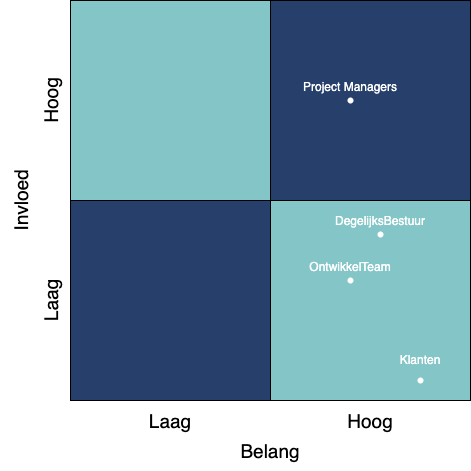
\includegraphics[width=10cm]{gfx/stakeholderanalyse}
    \caption{StakeHolders Analyse}
    \label{fig:StakeholderAnalyse1}
\end{figure}
Zoals te zien is in figuur~\ref{fig:StakeholderAnalyse1} is hebben alle stakeholders veel baat bij een nieuwe module voor de analyse van kwetsbaarheden. De invloed hierop is het hoogst bij het ontwikkelteam en de projectmanagers. De lage invloed van de klant zorgt ervoor dat voor het ontwerp alleen de requirements vanuit Eaglescience worden opgenomen.


\section{Requirements analyse}\label{sec:requirementsAnalyse}
Uit de opdracht van de CTO zijn er een aantal requirements die opgenomen dienen te worden in het nieuwe systeem. Hieronder volgt een lijst met daarbij een globale uitwerking hoe deze worden geimplementeerd. Ook zijn een aantal gerelateerde requirements samengevoegd. Getaileerde uitwerkingen zullen worden besproken in verdere hoofdstukken.

\subsection{Functionele eisen}\label{subsec:functionele-eisen}
De functionele eisen dienen direct te worden geïmplementeerd in het nieuwe systeem. en is daarom een onderdeel van het ontwerp dat in de komende hoofdstukken worden uitgewerkt.

\textbf{De module dient eenvoudig te kunnen worden gebruikt in de huidige Continuous Integration /Continuous Deployment (CI/CD) pipeline voor bestaande en nieuwe projecten.} De Tooling die gevonden is in het voorgaande onderzoek moeten worden geintegreert in de huidige manier van builden middels de Jenkins buildstraat. Er moet een concept komen waarin duidelijk is hoe de tooling wordt aangeroepen. Het doel van deze integratie is dat de informatie die beschikbaar wordt gebruikt kan worden in het nieuwe systeem. De informatie is gestructureerd middels JSON en dient in een data model te worden gegoten. Dit datamodel is vervolgens overal in het nieuwe systeem beschikbaar en zorgt ervoor dat de informatie uniform is. Daarnaast is het zaak om de integratie te doen op een generieke manier zodat in de toekomst toevoegingen kunnen worden toegevoegd voor het ondersteunen van andere platformen en talen zoals bijv Docker.


\textbf{De module dient te worden ontwikkeld in angular en Play(Scala) en gebruik te maken van de bestaande huidige projectstructuur van de portal} Eaglescience is al in het bezit van een portal waarin verschillende modulen beschikbaar zijn die de dagelijkse gang van zaken binnen het bedrijf toegankelijk maken. Het nieuwe systeem is hier een toevoeging op en dient dusdanig te worden opgebouwd dat deze naadloos aansluit bij de huidige modulen. Er moet dus uitgezocht worden hoe de portal is geimplementeerd en hoe het nieuwe systeem hierin samenvalt.

\textbf{De module dient ondersteuning te bieden aan meerdere omgevingen (OTAP)}
Door de tooling op meerdere plaatsen te integreren in de buildstraat kan er inzicht worden verschaft in het gebruik van externe bibliotheken op verschillende stadia van het ontwikkel process. Er moet dus een mechaniek worden ontwikkeld die het mogelijk maakt om op verschillende stadia van het process informatie over kwetsbaarheden in externe bibliotheken verschaft. Dit gegeven moet ook duidelijk in de interface worden weergegeven


\textbf{De module dient met een instelbaar interval de analyse uit te voeren} Door instellingen mechniscme in te bouwen en aan te bieden in de frontend kan er een interval worden opgegeven. Dit mechanisme kan ook worden ingezet voor allehande instellingen die per project verschillend zijn.
\textbf{De module moet op project en omgeving niveau rapporteren over bekende kwetsbaarheden} Twee views in de frontend moeten het mogelijk maken om rapporten in te zien op zowel project als omgevings niveau. Deze rapporten moeten ook worden verstuurt middels een notificatie(mail, rocket.chat etc.)

\textbf{De module dient kwetsbaarheden op minimaal drie niveau’s in te schalen (kritisch, gemiddeld en laag)}In de rapporten moet te zien zijn hoeveel kwetsbaarheden er van ieder niveau bestaan. Daarnaast moet er een allert komen op het moment dat er een instelbare grens wordt overschreden.

\section{Conclusie}\label{sec:conclusie}
%TODO: nodig......
